\documentclass[french, 11pt]{article}
\usepackage{amsmath}
\usepackage{amssymb}	% packages that allow mathematical formatting
\usepackage{graphicx}	% package that allows you to include graphics
\usepackage{setspace}	% package that allows you to change spacing
\usepackage{fullpage}	% package that specifies normal margins
\usepackage{microtype}
\usepackage{amsthm}
\newcommand{\argmin}{\operatornamewithlimits{argmin}}
\newcommand{\argmax}{\operatornamewithlimits{argmax}}
\usepackage{listings}
\usepackage{color}
\usepackage{caption}
\usepackage{subcaption}
\usepackage{rotating} % Rotating table
\usepackage{enumerate}
\usepackage{graphicx}               % Necessary to use \scalebox
\usepackage{amsmath,amssymb}

\definecolor{codegreen}{rgb}{0,0.6,0}
\definecolor{codegray}{rgb}{0.5,0.5,0.5}
\definecolor{codepurple}{rgb}{0.58,0,0.82}
\definecolor{backcolour}{rgb}{0.95,0.95,0.95}




\usepackage[left=2.5cm, right=2.5cm, top=2cm, bottom = 3cm]{geometry}




\begin{document}
\noindent Patrick Shultz\\
\noindent FNCE 921 Assignment 3\\
\today\\

\section{Factor Models}
\paragraph{a)} Use monthly data on the univariate size-sorted portfolios and book-to-market sorted decile portfolios to etimate alphas and betas, as well as compute the GRS test statistics to test the CAPM and Fama-French 3 factor model.\\

\noindent\textbf{Solution:} Fama and French consider regressions of the form
\begin{equation}
\begin{split}
R^{ei}_t = \alpha_{i} + \beta_i f_t + \epsilon_{it}, \quad t = 1, 2, ... T \forall i
\end{split}
\label{eq:FF_regressions}
\end{equation}
Where $R^e$ denotes an excess return and $f$ is a factor portfolio, which is an excess return. These time series regressions directly imply
\begin{equation*}
E(R^{ei}) = \alpha_{i} + \beta_i E(f)
\end{equation*}
by taking averages. CAPM uses the excess return as the only factor. We can then implement Equation \ref{eq:FF_regressions} for each portfolio. We get the estimates shown in Table \ref{tab:CAPM_estimates}, which show that $\beta$'s and returns go in the correct direction. However, the test of whether or not CAPM works is a test of whether or not the intercepts are jointly equal to zero. 

\begin{table}[!htbp] \centering 
	\caption{CAPM Test for Size and Book-to-Market Portfolios (Full Sample)} 
	\label{} 
	\begin{tabular}{@{\extracolsep{5pt}} c|ccc||ccc} 
		\\[-1.8ex]\hline 
		\hline \\[-1.8ex] 
		&\multicolumn{3}{c}{Size estimates} & \multicolumn{3}{c}{BE/ME estimates}\\
		& $\alpha$ & $\beta$ & E(R) & $\alpha$ & $\beta$ & E(R) \\ 
		\hline \\[-1.8ex] 
		d1 & $0.451$ & $1.414$ & $1.384$ & $0.207$ & $1.009$ & $0.873$ \\ 
		d2 & $0.342$ & $1.381$ & $1.254$ & $0.347$ & $0.945$ & $0.971$ \\ 
		d3 & $0.370$ & $1.325$ & $1.245$ & $0.334$ & $0.966$ & $0.972$ \\ 
		d4 & $0.382$ & $1.254$ & $1.209$ & $0.244$ & $1.043$ & $0.933$ \\ 
		d5 & $0.351$ & $1.226$ & $1.160$ & $0.340$ & $1.000$ & $1.000$ \\ 
		d6 & $0.380$ & $1.201$ & $1.173$ & $0.385$ & $1.027$ & $1.063$ \\ 
		d7 & $0.343$ & $1.149$ & $1.102$ & $0.260$ & $1.096$ & $0.984$ \\ 
		d8 & $0.341$ & $1.111$ & $1.074$ & $0.433$ & $1.136$ & $1.183$ \\ 
		d9 & $0.304$ & $1.060$ & $1.004$ & $0.478$ & $1.275$ & $1.320$ \\ 
		d10 & $0.272$ & $0.928$ & $0.885$ & $0.355$ & $1.459$ & $1.318$ \\ 
		\hline \\[-1.8ex] 
	\end{tabular}
\label{tab:CAPM_estimates}
\end{table}
The GRS test statistic allows us to test the hypothesis $\alpha_i = 0\quad \forall i$. The GRS test is given by 
\begin{equation*}
	\left(\dfrac{T}{N}\right)\left(\dfrac{T-N-L}{T-L-1}\right)\left[\frac{\hat{\alpha}'\hat{\Sigma}^{-1}\hat{\alpha}}{1 + \bar{f}'\hat{\Omega}^{-1}\bar{f}}\right] \sim F(N, T-N-L)
\end{equation*} 
where $\hat{\alpha}$ is a $N\times 1$ vector of estimated intercepts, $\hat{\Sigma}$ is an unbiased estimate of the residual covariance matrix, $\bar{f}$ is a $L\times 1$ vector of the factor portfolios' covariance matrix. Hence in our case, the GRS statistic will be distributed as $F(10, T-10-1)$. The critical value for $\%95$ confidence for this distribution in 1.84. We get GRS test statistics of 35.77 and 72.36 for book to market and size, respectively. Hence, we can reject the null hypothesis that the $\alpha$'s are jointly zero are the $\%95$ confidence level. \\

Next we consider the Fama-French 3 factor model
\begin{equation*}
	R^{ei}_t = \alpha_i + b_i(R_{Mt} - R_{ft}) + s_i(SMB_t) + h_i(HML_t) + \epsilon_{it}
\end{equation*}
\begin{table}[!htbp] \centering 
	\caption{} 
	\label{} 
	\begin{tabular}{@{\extracolsep{5pt}} c|ccc||ccc} 
		\\[-1.8ex]\hline 
		\hline \\[-1.8ex] 
		&\multicolumn{3}{c}{Size estimates} & \multicolumn{3}{c}{BE/ME estimates}\\
		& $\alpha$ & $\beta$ & E(R) & $\alpha$ & $\beta$ & E(R) \\ 
		\hline \\[-1.8ex] 
		d1 & $0.301$ & $1.074$ & $0.873$ & $0.118$ & $0.997$ & $1.384$ \\ 
		d2 & $0.397$ & $0.975$ & $0.971$ & $0.112$ & $1.065$ & $1.254$ \\ 
		d3 & $0.350$ & $0.982$ & $0.972$ & $0.189$ & $1.076$ & $1.245$ \\ 
		d4 & $0.206$ & $1.027$ & $0.933$ & $0.228$ & $1.038$ & $1.209$ \\ 
		d5 & $0.275$ & $0.975$ & $1.000$ & $0.241$ & $1.059$ & $1.160$ \\ 
		d6 & $0.277$ & $0.973$ & $1.063$ & $0.281$ & $1.071$ & $1.173$ \\ 
		d7 & $0.114$ & $1.008$ & $0.984$ & $0.274$ & $1.050$ & $1.102$ \\ 
		d8 & $0.247$ & $1.012$ & $1.183$ & $0.291$ & $1.048$ & $1.074$ \\ 
		d9 & $0.237$ & $1.104$ & $1.320$ & $0.268$ & $1.030$ & $1.004$ \\ 
		d10 & $0.024$ & $1.190$ & $1.318$ & $0.298$ & $0.974$ & $0.885$ \\ 
		\hline \\[-1.8ex] 
	\end{tabular} 
\end{table} 

We can repeat this analysis for the past 10 years and past 25 years. The  GRS test statistics and associated critical F-values are shown in \ref{tab:GRS_table}
\begin{table}[!htbp] \centering 
	\caption{GRS Statistics} 
	\label{tab:GRS_table} 
	\begin{tabular}{@{\extracolsep{5pt}} cccc} 
		\\[-1.8ex]\hline 
		\hline \\[-1.8ex] 
		& BE/ME & Size & Critical Value ($\%95$) \\ 
		\hline \\[-1.8ex] 
		CAPM (Full Sample) & $35.771$ & $72.363$ & $1.839$ \\ 
		FF3 (Full Sample) & $35.792$ & $85.591$ & $1.839$ \\ 
		CAPM (Last 10 Years) & $2.747$ & $2.176$ & $1.839$ \\ 
		FF3 (Last 10 Years) & $280.745$ & $209.916$ & $1.839$ \\ 
		CAPM (Last 25 Years) & $8.520$ & $599.408$ & $1.839$ \\ 
		FF3 (Last 25 Years) & $138.727$ & $292.573$ & $1.839$ \\ 
		\hline \\[-1.8ex] 
	\end{tabular} 
\end{table} 
Hence, we strongly reject the model in all samples. \\

\paragraph{b)} Run Fama-MacBeth cross-sectional regressions of excess returns on the Fama-French factors as well as the two characteristics: Size and average Book/Market. Do the latter  have significant slope coefficients? Do the results change if you omit the SMB and HML factors from the regression. 

\noindent \textbf{Solution:} We use the following procedure 
\begin{enumerate}
	\item Run the time series regressions: $R^{ei}_{t} = a_{i} + \beta'_{i}f_{t} + \epsilon_{it}$. In this case $f = \left[R^{m}-R^{f}, \text{SMB}, \text{HML}\right]$. 
	\item Then we run the cross-section as a separate regression for each $t$: $R^{ei}_t =  \beta'_{i}\lambda_{t} + \alpha_{it}$, where $\beta$ from step 1 is the right hand side variable and $\lambda$ (the price of risk) is the coefficient to be estimated. We get a different price of risk and error term for each $t$. Where we can include size and book/market as additional characteristics. 
	\item Estimate the price of risk as $\hat{\lambda}_t = E_T(\hat{\lambda}_{t})$ and $\hat{\alpha} = E_T(\hat{\alpha}_{T})$
	\item Estimate the standard errors as $\sigma(\hat{\lambda}) = \frac{\sigma(\hat{\lambda}_{t})}{\sqrt{T}}$.
\end{enumerate}
\begin{table}[!htbp] \centering 
	\caption{Fama-MacBeth Slope Coefficients} 
	\label{} 
	\begin{tabular}{@{\extracolsep{5pt}} cccccc} 
		\\[-1.8ex]\hline 
		\hline \\[-1.8ex] 
		& RX & SMB & HML & ln(Size) & ln(BE/ME) \\ 
		\hline \\[-1.8ex] 
		lambda.size. & $0.136$ & $$-$0.113$ & $$-$0.002$ & $3.654$ & $$-$0.364$ \\ 
		t.lambda. & $4.596$ & $$-$1.730$ & $$-$0.070$ & $3.123$ & $$-$2.571$ \\ 
		lambda.BE.ME. & $0.083$ & $0.019$ & $0.051$ & $5.055$ & $$-$0.369$ \\ 
		t.lambda..1 & $3.380$ & $0.340$ & $2.447$ & $3.363$ & $$-$2.025$ \\ 
		\hline \\[-1.8ex] 
	\end{tabular} 
\end{table} 
Hence, we see that including that size and book to market ratios are significant. We can reestimate the  parameters with a specification that leaves these out and get the following. 
\begin{table}[!htbp] \centering 
	\caption{Fama-MacBeth Slope Coefficients} 
	\label{} 
	\begin{tabular}{@{\extracolsep{5pt}} cccc} 
		\\[-1.8ex]\hline 
		\hline \\[-1.8ex] 
		& RX & SMB & HML \\ 
		\hline \\[-1.8ex] 
		lambda.size. & $0.157$ & $$-$0.131$ & $$-$0.006$ \\ 
		t.lambda. & $4.885$ & $$-$3.233$ & $$-$0.304$ \\ 
		lambda.BE.ME. & $0.114$ & $$-$0.019$ & $0.047$ \\ 
		t.lambda..1 & $5.619$ & $$-$0.448$ & $2.346$ \\ 
		\hline \\[-1.8ex] 
	\end{tabular} 
\end{table} 
Results generally do not change when we omit the size and book to market factors. 

\paragraph{c)} Download (real) aggregate nondurable and services consumption from BEA or FRED, at monthly and quarterly frequencies. Test the standard consumption-based CAPM, using both Fama-MacBeth cross-sectional regressions and SDF-GMM methods, report estimates of cross-sectional factor risk premia ($\lambda$'s) and SDF loadings ($b$'s) and their standard errors, as well as the relevant cross-sectional tests. Is the model rejected? What is the price of consumption risk that is implied by this cross-section of asset returns? Plot the actual mean excess returns against the predicted excess returns. \\

\noindent\textbf{Solution:} The CCAPM states
\begin{equation*}
	E\left[R^{ei}\right] = \gamma cov(\Delta c_{t+1}, R^{ei}_{t+1}) = \dfrac{cov(\Delta c_{t+1}, R^{ei}_{t+1})}{var(\Delta c_{t+1})}\left[\gamma var(\Delta c_{t+1})\right]= \beta_{i, M}\lambda_{\Delta c}
\end{equation*}
It states that the expected return of asset $i$ is proportional to beta times the market price of consumption risk. This representation implies we can run the following test of the model 
\begin{equation*}
	\begin{split}
	R^{ei}_{t+1} &= a_{i} + \beta_{i, \Delta c}\Delta c_{t+1} + \epsilon^{i}_{t+1} \quad t = 1,..., T\\
	E(R^{ei}) &= \beta_{i, \Delta c} \lambda_{\Delta c} + \alpha_{i}
	\end{split}
\end{equation*}
In the first stage the point is to estimate the tendency for the asset to fall when consumption falls (i.e. estimate $\beta$). The second stage is the test of the statement of the model: $\alpha$'s should be zero and we should see expected return to be high where $\beta$'s are high. We get the following results 
\begin{table}[!htbp] \centering 
	\caption{} 
	\label{} 
	\begin{tabular}{@{\extracolsep{5pt}} c|cccccccccc} 
		\\[-1.8ex]\hline 
		\hline \\[-1.8ex] 
		& d1 & d2 & d3 & d4 & d5 & d6 & d7 & d8 & d9 & d10 \\ 
		\hline \\[-1.8ex] 
		E(R) size & $1.033$ & $1.003$ & $1.073$ & $1.027$ & $1.038$ & $1.018$ & $1.021$ & $1.005$ & $0.965$ & $0.870$ \\ 
		alpha size & $0.179$ & $0.200$ & $0.315$ & $0.295$ & $0.295$ & $0.417$ & $0.366$ & $0.418$ & $0.415$ & $0.297$ \\ 
		beta size & $1.220$ & $1.147$ & $1.082$ & $1.044$ & $1.062$ & $0.858$ & $0.936$ & $0.838$ & $0.785$ & $0.819$ \\ \hline
		E(R) BE/ME & $0.844$ & $0.916$ & $0.926$ & $0.899$ & $0.982$ & $1.033$ & $0.920$ & $1.109$ & $1.168$ & $1.165$ \\ 
		alpha BE/ME & $0.213$ & $0.286$ & $0.396$ & $0.417$ & $0.500$ & $0.402$ & $0.287$ & $0.469$ & $0.538$ & $0.263$ \\ 
		beta BE/ME & $0.901$ & $0.900$ & $0.758$ & $0.689$ & $0.689$ & $0.902$ & $0.905$ & $0.914$ & $0.900$ & $1.289$ \\ 
		\hline \\[-1.8ex] 
	\end{tabular} 
\end{table} \\
\begin{figure}[!htb]
	\centering
	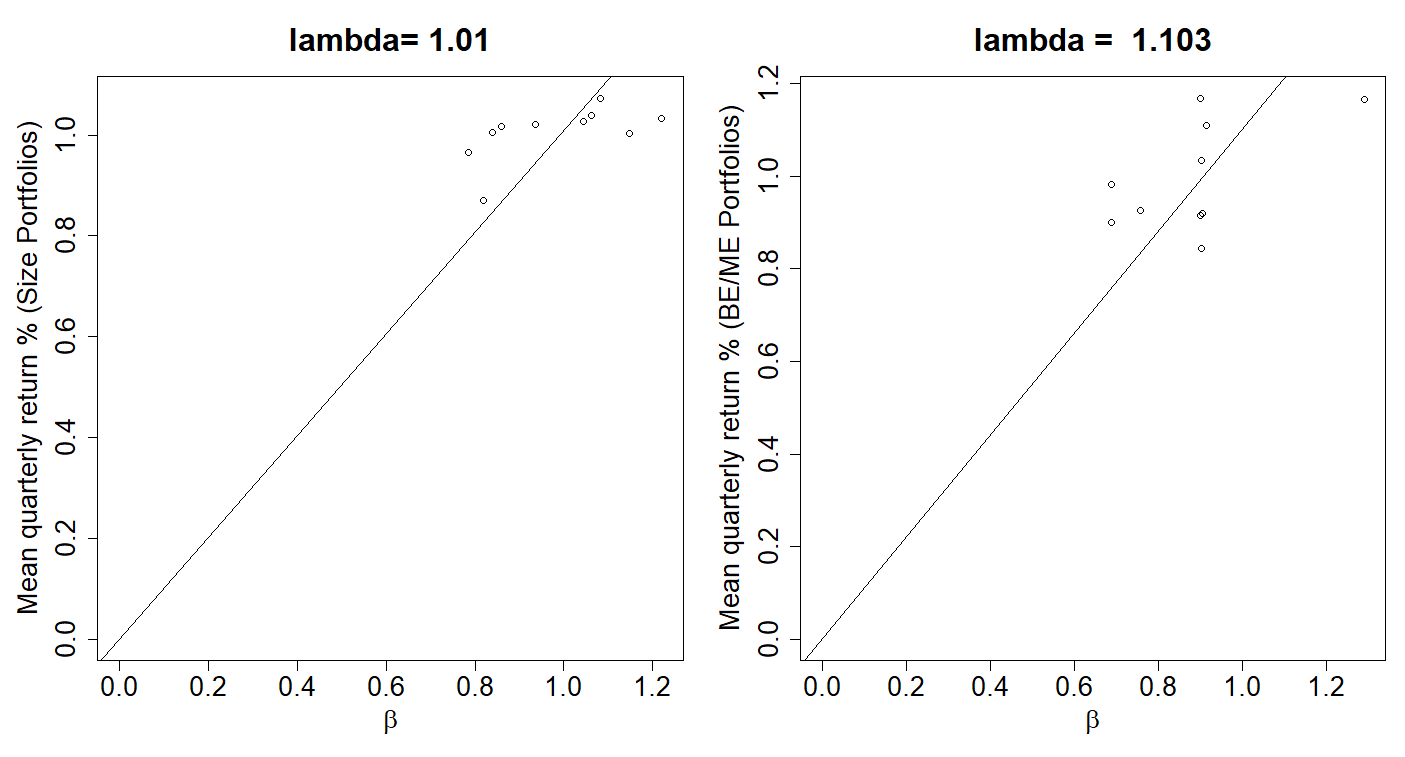
\includegraphics[width=0.9\linewidth]{FM_ccapm.png}
	\caption{Fama MacBeth tests of the CCAPM}
	\label{fig:FMB_CCAPM}
\end{figure}\\

 
An alternative way to deal with the generated regressor problem is to use GMM to estimate $a, \beta$, and $\lambda$. The CCAPM has a single factor, namely $f = \Delta c_{t+1}$. Then the moment conditions are
$$
	g_{T} = 
	\begin{bmatrix}
	E(R_{t}^{e} - a - \beta f_{t})\\
	E\left[(R^{e}_{t}-a-\beta f_{t})f_{t}\right]\\
	E(R^{e} - \beta \lambda)
	\end{bmatrix}
	=
	\begin{bmatrix}
	0\\ 0 \\ 0
	\end{bmatrix}
$$
The top two moment conditions identify $a$ and $\beta$ as the time-series OLS estimates and the bottom moment condition is implied by our asset pricing model. The parameter vector is $\theta' = \left[a'\quad \beta'\quad \lambda \right]$ Define the matrix $d$ as the sensitivity of the moment conditions to the parameters. 
$$
d = \dfrac{\partial g_{T}}{\partial b'}
$$

%Using GMM, we use the following procedure to compute the SDF loadings
%\begin{equation*}
%	\begin{split}
%	0 &= E(MR^e)\\
%	M &= 1-b'(f-Ef) = 1-b'\tilde{f} \\
%	g_T &= E_T\left[R^e(1-b\tilde{f})\right]\\
%	d &= \frac{\partial g_t}{\partial b}-E(R^e\tilde{f}')=-cov(R^e, f') = -c\\
%	\min& g_t'Wg_t \implies \text{FOC:  } d'Wg_t = 0\\
%	0&=d'W E_T(R^e(1-\tilde{f}'b))\implies 0=-c'W E_T(R^e(1-\tilde{f}'b))\\
%	& c'WE_T(R^e) = c'Wcb\\
%	b &= \left[c'Wc\right]^{-1}c'WE_T(R^e)\\
%	\end{split}
%\end{equation*}
%In the case of CCAPM the factor, $f$,  is consumption growth, $\Delta c_{t+1}$, so we see that GMM is just a cross sectional regression of expected returns on covariances. That is, GMM is equivalent to considering the cross-sectional model $E(R^{e}) = cov(R^{e}, \Delta c_{t+1}) b$, where we can just run a GLS regression to estimate $b$. We can rewrite this in terms of regression coefficients to make our estimates comparable
%\begin{equation*}
%	E(R^{e}) = \dfrac{cov(R^{e}, \Delta c_{t+1})}{var(\Delta c_{t+1})}(var(\Delta c_{t+1})b) = b_{i, \Delta c}\lambda_{\Delta c}
%\end{equation*}

\end{document}
